\subsection{General information}
\begin{frame}
	\frametitle{Proton Accelerator at Paul Scherrer Institute (PSI)}
	\begin{itemize}
		\setlength{\itemsep}{\fill}
		\item High Intensity Proton Accelerator (HIPA) at PSI (Cyclotron)
		\item \SI{590}{\mega\electronvolt} proton beam with beam current up to \SI{2.4}{\milli\ampere} (\SI{1.5e16}{protons\per s})
		\begin{itemize}
			\vspace*{4pt}
			\item \SI{\sim1.4}{\mega\watt} \ra most powerful proton accelerator in the world
		\end{itemize}
		\vspace*{4pt}
		\item only two comparable accelerators
		\begin{itemize}
			\vspace*{4pt}
			\item TRIUMF in Vancouver (\SI{\sim0.25}{\mega\watt})
			\item LAMPF in Los Alamos (\SI{\sim0.8}{\mega\watt})
		\end{itemize}
% 		\item LHC takes \SI{28}{\minute} to accelerate a full injection (\SI{\sim0.2}{\mega\watt})
	\end{itemize}
	\begin{figure}
		\centering
		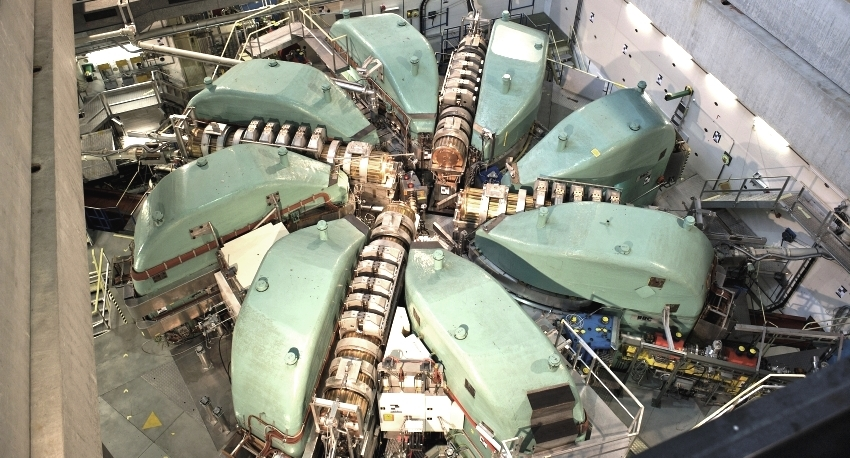
\includegraphics[width=6.5cm]{cyclotron}
	\end{figure}
\end{frame}
% ============================ new frame ==========================================>
\begin{frame}
	\frametitle{Beam line at Paul Scherrer Institute (PSI)}
	\begin{minipage}[c][.75\textheight]{6.5cm}
		\begin{itemize}
			\setlength{\itemsep}{\fill}
			\item using beam line $\uppi$M1 with \SI{260}{\mega\electronvolt\per c} positive pions ($\uppi^+$)
			\item tunable particle fluxes from \SI{2}{\kilo\hertz\per cm^2} to \SI{10}{\mega\hertz\per cm^2}
		\end{itemize}
		\begin{figure}
			\centering
			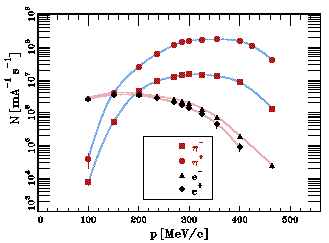
\includegraphics[width=5cm]{pim1}
		\end{figure}
	\end{minipage}
	\begin{minipage}{4.5cm}
		\begin{figure}
			\centering
			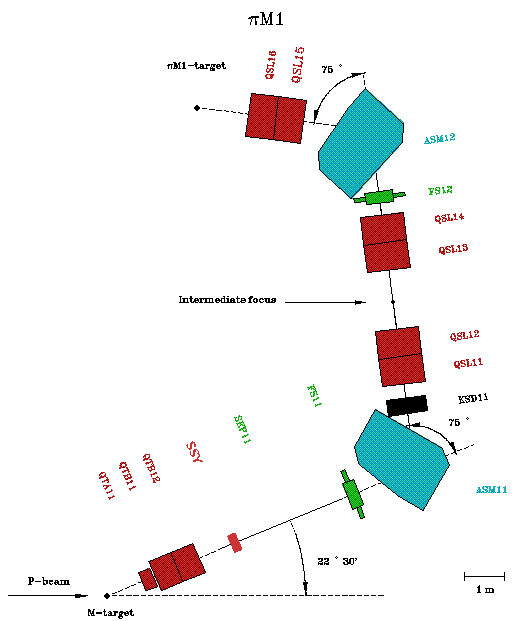
\includegraphics[width=5cm]{bpim1}
		\end{figure}
	\end{minipage}
\end{frame}
% ============================ new frame ==========================================>
\begin{frame}
	\frametitle{Measurements}
	\begin{itemize}
		\item performing several beam tests starting in $2013$
		\item using a modular self-built beam telescope with two possible setups:
			\begin{itemize}
				\item pad setup (testing whole diamonds as single pad detector)
				\item pixel setup (testing diamond sensors implanted on CMS-Pixel Chips)
			\end{itemize}
		\item investigating several materials and devices
		\begin{itemize}
			\item scCVD pad detectors (reproduce rate effect)
			\item pCVD pad and pixel detectors
			\item very first 3D pixel detector
		\end{itemize}
		\item studying non-irradiated and irradiated devices (up to \SI{2e15}{neq\per cm^2})
	\end{itemize}
	\begin{figure}
		\centering
		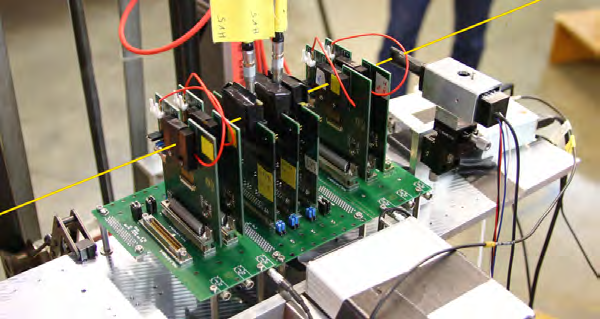
\includegraphics[width=6cm]{pad}
	\end{figure}
\end{frame}